\documentclass{beamer}
\usetheme{Boadilla}  %% Themenwahl

\title{Freie Theoreme}
\author{Thomas Rossow}
\date{23. November 2016}

\usepackage[utf8]{inputenc} % set input encoding (not needed with XeLaTeX)

\AtBeginSection[]{
  \begin{frame}
  \vfill
  \centering
  \begin{beamercolorbox}[sep=8pt,center,shadow=true,rounded=true]{title}
    \usebeamerfont{title}\insertsectionhead\par%
  \end{beamercolorbox}
  \vfill
  \end{frame}
}

\beamertemplatenavigationsymbolsempty
\setbeamertemplate{footline}{\hfill\makebox[24pt]{\scriptsize\insertframenumber/\inserttotalframenumber}}

\begin{document}
\maketitle
\frame{\tableofcontents}

\section{Was sind freie Theoreme?}

\begin{frame}
\frametitle{Gib mir eine Signatur...}
\begin{center}
\texttt{f :: [a] $\rightarrow$ [a]}
\end{center}
\end{frame}

\begin{frame}
\frametitle{Gib mir eine Signatur...}
\begin{center}
\texttt{f :: [a] $\rightarrow$ [a]}

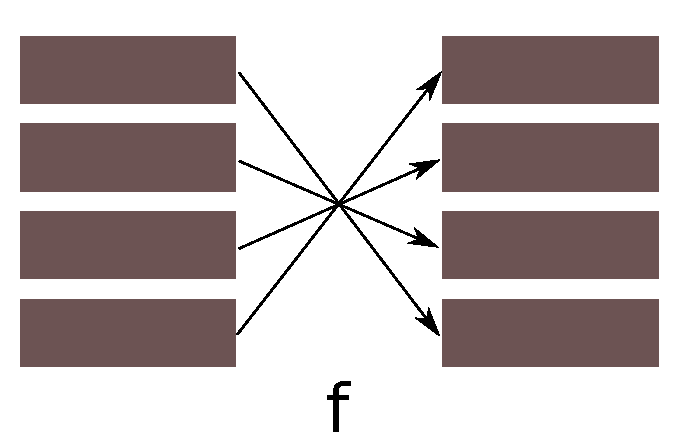
\includegraphics[width=200px]{list-order-blank}
\end{center}
\end{frame}

\begin{frame}
\frametitle{Gib mir eine Signatur...}
\begin{center}
\texttt{f :: [a] $\rightarrow$ [a]}

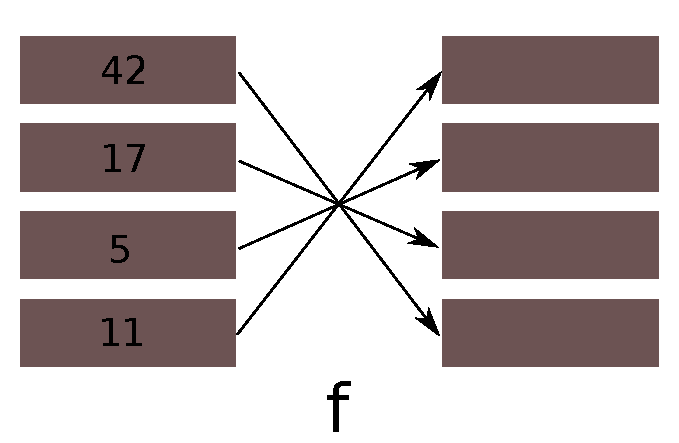
\includegraphics[width=200px]{list-order-onlyleft}
\end{center}
\end{frame}

\begin{frame}
\begin{center}
\frametitle{Gib mir eine Signatur...}
\texttt{f :: [a] $\rightarrow$ [a]}

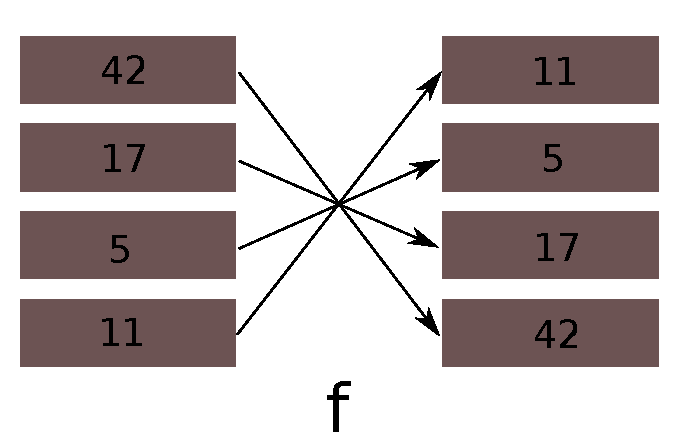
\includegraphics[width=200px]{list-order}
\end{center}
\end{frame}

\begin{frame}
\frametitle{Gib mir eine Signatur...}
\begin{center}
\texttt{g :: Int $\rightarrow$ Int}

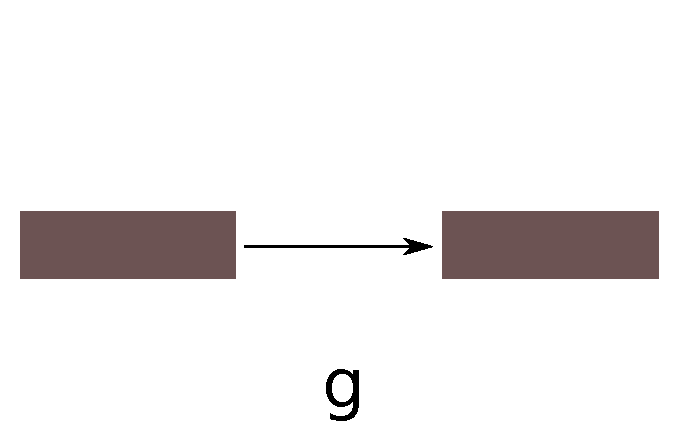
\includegraphics[width=150px]{g-function-blank}
\end{center}
\end{frame}

\begin{frame}
\frametitle{Gib mir eine Signatur...}
\begin{center}
\texttt{g :: Int $\rightarrow$ Int}

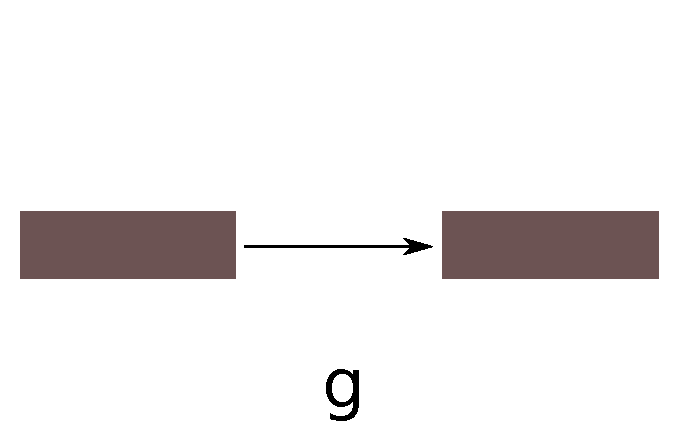
\includegraphics[width=150px]{g-function}
\end{center}
\end{frame}

\begin{frame}
\frametitle{Gib mir eine Signatur...}
%\texttt{f :: [a] $\rightarrow$ [a]}

\begin{center}
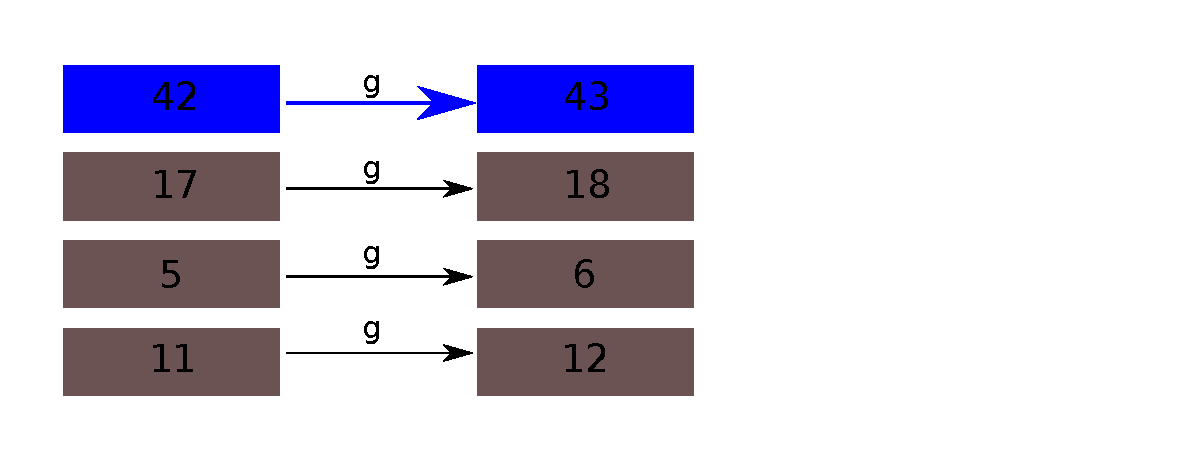
\includegraphics[width=250px]{mapg}
\end{center}
\end{frame}

\begin{frame}
\frametitle{Gib mir eine Signatur...}
%\texttt{f :: [a] $\rightarrow$ [a]}
\begin{center}
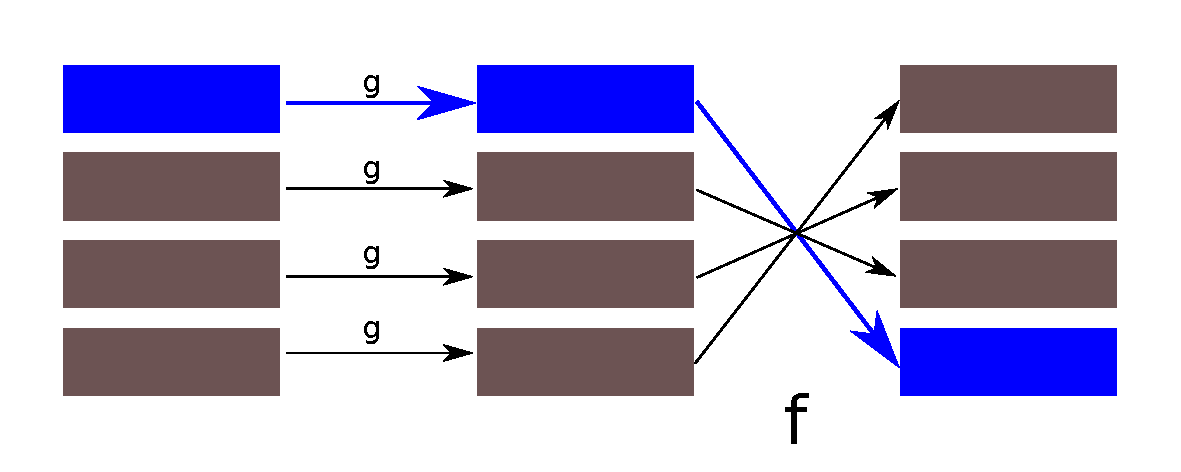
\includegraphics[width=250px]{mapgf}
\end{center}
\end{frame}

\begin{frame}
\frametitle{Gib mir eine Signatur...}
%\texttt{f :: [a] $\rightarrow$ [a]}

\begin{center}
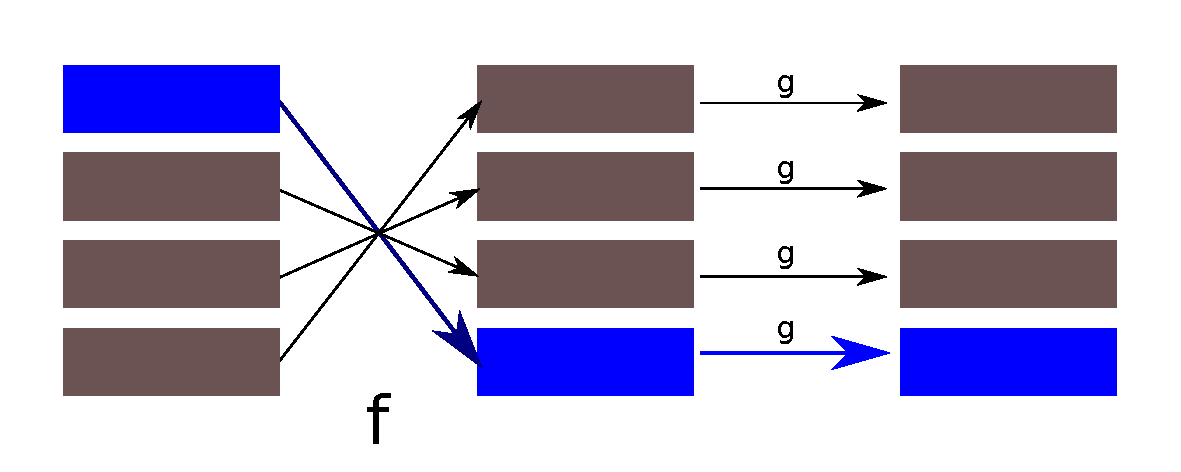
\includegraphics[width=250px]{fmapg}
\end{center}
\end{frame}

\begin{frame}
\frametitle{...und ich schenke dir ein Theorem}
\begin{center}
\texttt{f :: [a] $\rightarrow$ [a]}

\begin{align*}
f\ (map\ g\ l) = map\ g\ (f\ l)
\end{align*}

Für alle Listen \texttt{l} und alle Funktionen \texttt{g}.

\end{center}
\end{frame}

\section{Die Theorie dahinter}
\begin{frame}
\frametitle{Die Theorie dahinter}

\begin{itemize}
\item Grundgedanke: Typen als Relationen
\item Basistypen: Identitätsrelationen
\item Komplexe Typen: Konstruktion aus Relationen
\end{itemize}

\end{frame}

\begin{frame}
\frametitle{Die Theorie dahinter}

Beispiel: Bool (Basistyp)

\begin{align*}
&\mathcal{R} : Bool \Leftrightarrow Bool\\
&\mathcal{R} = \{ (True, True), (False, False) \}
\end{align*}

\end{frame}

%\begin{frame}
%\frametitle{Die Theorie dahinter}
%
%Beispiel: $\mathcal{R} \rightarrow \mathcal{S}$ (Funktionskonstruktor)
%
%\begin{align*}
%&(f, g) \in \mathcal{R} \rightarrow \mathcal{S}\\
%&\\
%:\Leftrightarrow &
%\forall (x, y) \in \mathcal{R}:\\
%&(f\ x, g\ y) \in \mathcal{S}
%\end{align*}
%
%
%\end{frame}

\begin{frame}
\frametitle{Die Theorie dahinter}

Beispiel: $\forall \mathcal{X} . \mathcal{F}(\mathcal{X})$ (Allquantifizierung)

\begin{align*}
&(f, g) \in \forall \mathcal{X} . \mathcal{F}(\mathcal{X})\\
&\\
:\Leftrightarrow &
\forall T_1, T_2 \in Types, \mathcal{A} : T_1 \Leftrightarrow T_2:\\
&(f_{T_1}, g_{T_2}) \in \mathcal{F}(\mathcal{A})
\end{align*}


\end{frame}

\begin{frame}
\frametitle{Die Theorie dahinter}

\begin{Theorem}[Parametrizität]
Ist e ein Ausdruck vom Typ t (also e :: t) und ist $\mathcal{R}$ die zu t konstruierte Typrelation, so gilt
$(e, e) \in \mathcal{R}$.
\end{Theorem}

\end{frame}

\begin{frame}
\frametitle{Die Theorie dahinter}

\begin{itemize}
\item Parametrizität liefert Aussage zu jeder Typsignatur
\item Abrollen der Relationsdefinitionen führt zu Theorem
\end{itemize}

\end{frame}

\begin{frame}
\frametitle{Die Theorie dahinter}

\texttt{f :: [a] $\rightarrow$ [a]}

\begin{align*}
(f, f) \in \forall \mathcal{R} . [\mathcal{R}] \rightarrow [\mathcal{R}]
\end{align*}

\end{frame}

\begin{frame}
\frametitle{Typkonstruktorvariablen}
\texttt{fmap :: Functor f => (a $\rightarrow$ b) $\rightarrow$ f\ a $\rightarrow$ f\ b}

\begin{itemize}
\item \texttt{f} ist von der Sorte $* \rightarrow *$.
\end{itemize}
\end{frame}

\begin{frame}
\frametitle{Typkonstruktorvariablen}

\texttt{fmap :: Functor f => (a $\rightarrow$ b) $\rightarrow$ f\ a $\rightarrow$ f\ b}

\begin{align*}
&\forall k1, k2 \in (* \rightarrow *), \mathcal{K} : k_1 \Leftrightarrow k_2, \mathcal{K}\ respects\ Functor \\
&\forall A, A' \in Typen, \mathcal{A} : A \Leftrightarrow A' \\
&\forall B, B' \in Typen, \mathcal{B} : B \Leftrightarrow B' \\
&\forall (g, g') \in (\mathcal{A} \rightarrow \mathcal{B}) \\
&(\forall (x, x') \in \mathcal{A}: (g\ x, g'\ x') \in \mathcal{B})\\
&\Rightarrow (\forall (y, y') \in \mathcal{K} \mathcal{A} \\
&\ \ \ \ \ \ fmap_{k1 A B}\ g\ y, fmap_{k2 A' B'}\ g'\ y') \in \mathcal{K} \mathcal{B}\\
\end{align*}
\end{frame}

\begin{frame}
\frametitle{Typkonstruktorvariablen}
\begin{itemize}
\item Ähnlich wie Allquantifizierung über Typvariablen
\item Funktionen auf Relationen
\item Implementierung möglich
\end{itemize}
\end{frame}

\begin{frame}
\frametitle{Anwendungsbeispiel: Funktorgesetze}

\begin{texttt}
1. fmap id      = id\\
2. fmap (p . q) = (fmap p) . (fmap q)
\end{texttt}

\begin{itemize}
\item Tatsächlich folgt 2. aus 1. und Parametrizität
\end{itemize}

\end{frame}

\section{Die Bibliothek free-theorems}

\begin{frame}
\frametitle{Überblick}
\begin{columns}
\begin{column}{0.4\textwidth}
    \begin{center}
	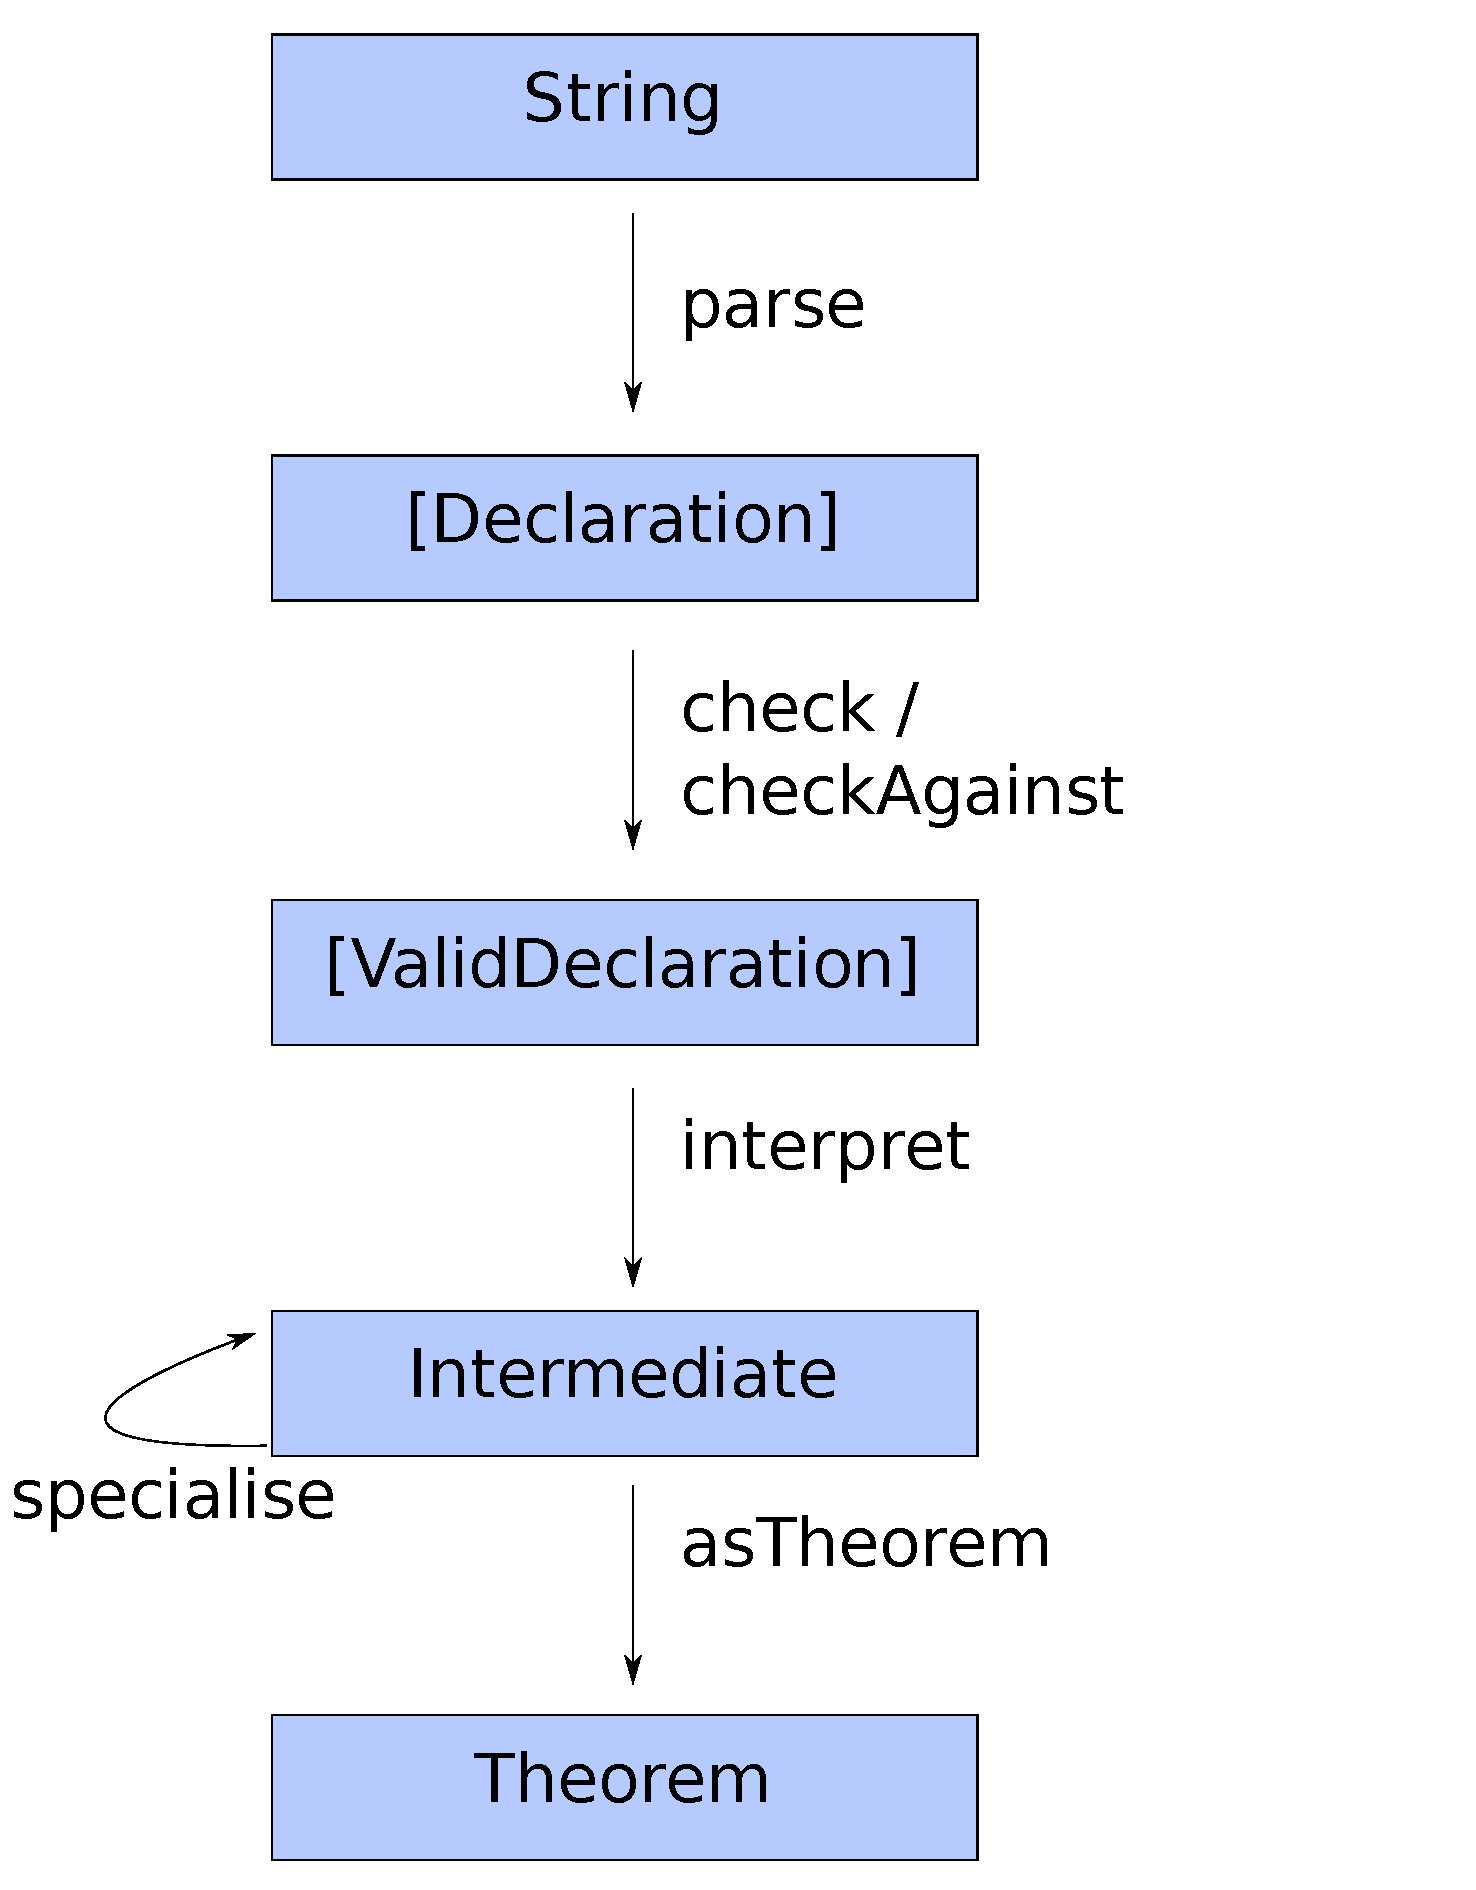
\includegraphics[height=200px]{overview-free-theorems}
     \end{center}
\end{column}
\begin{column}{0.6\textwidth}
\end{column}
\end{columns}
\end{frame}

\begin{frame}
\frametitle{Überblick}
\begin{columns}
\begin{column}{0.4\textwidth}
    \begin{center}
	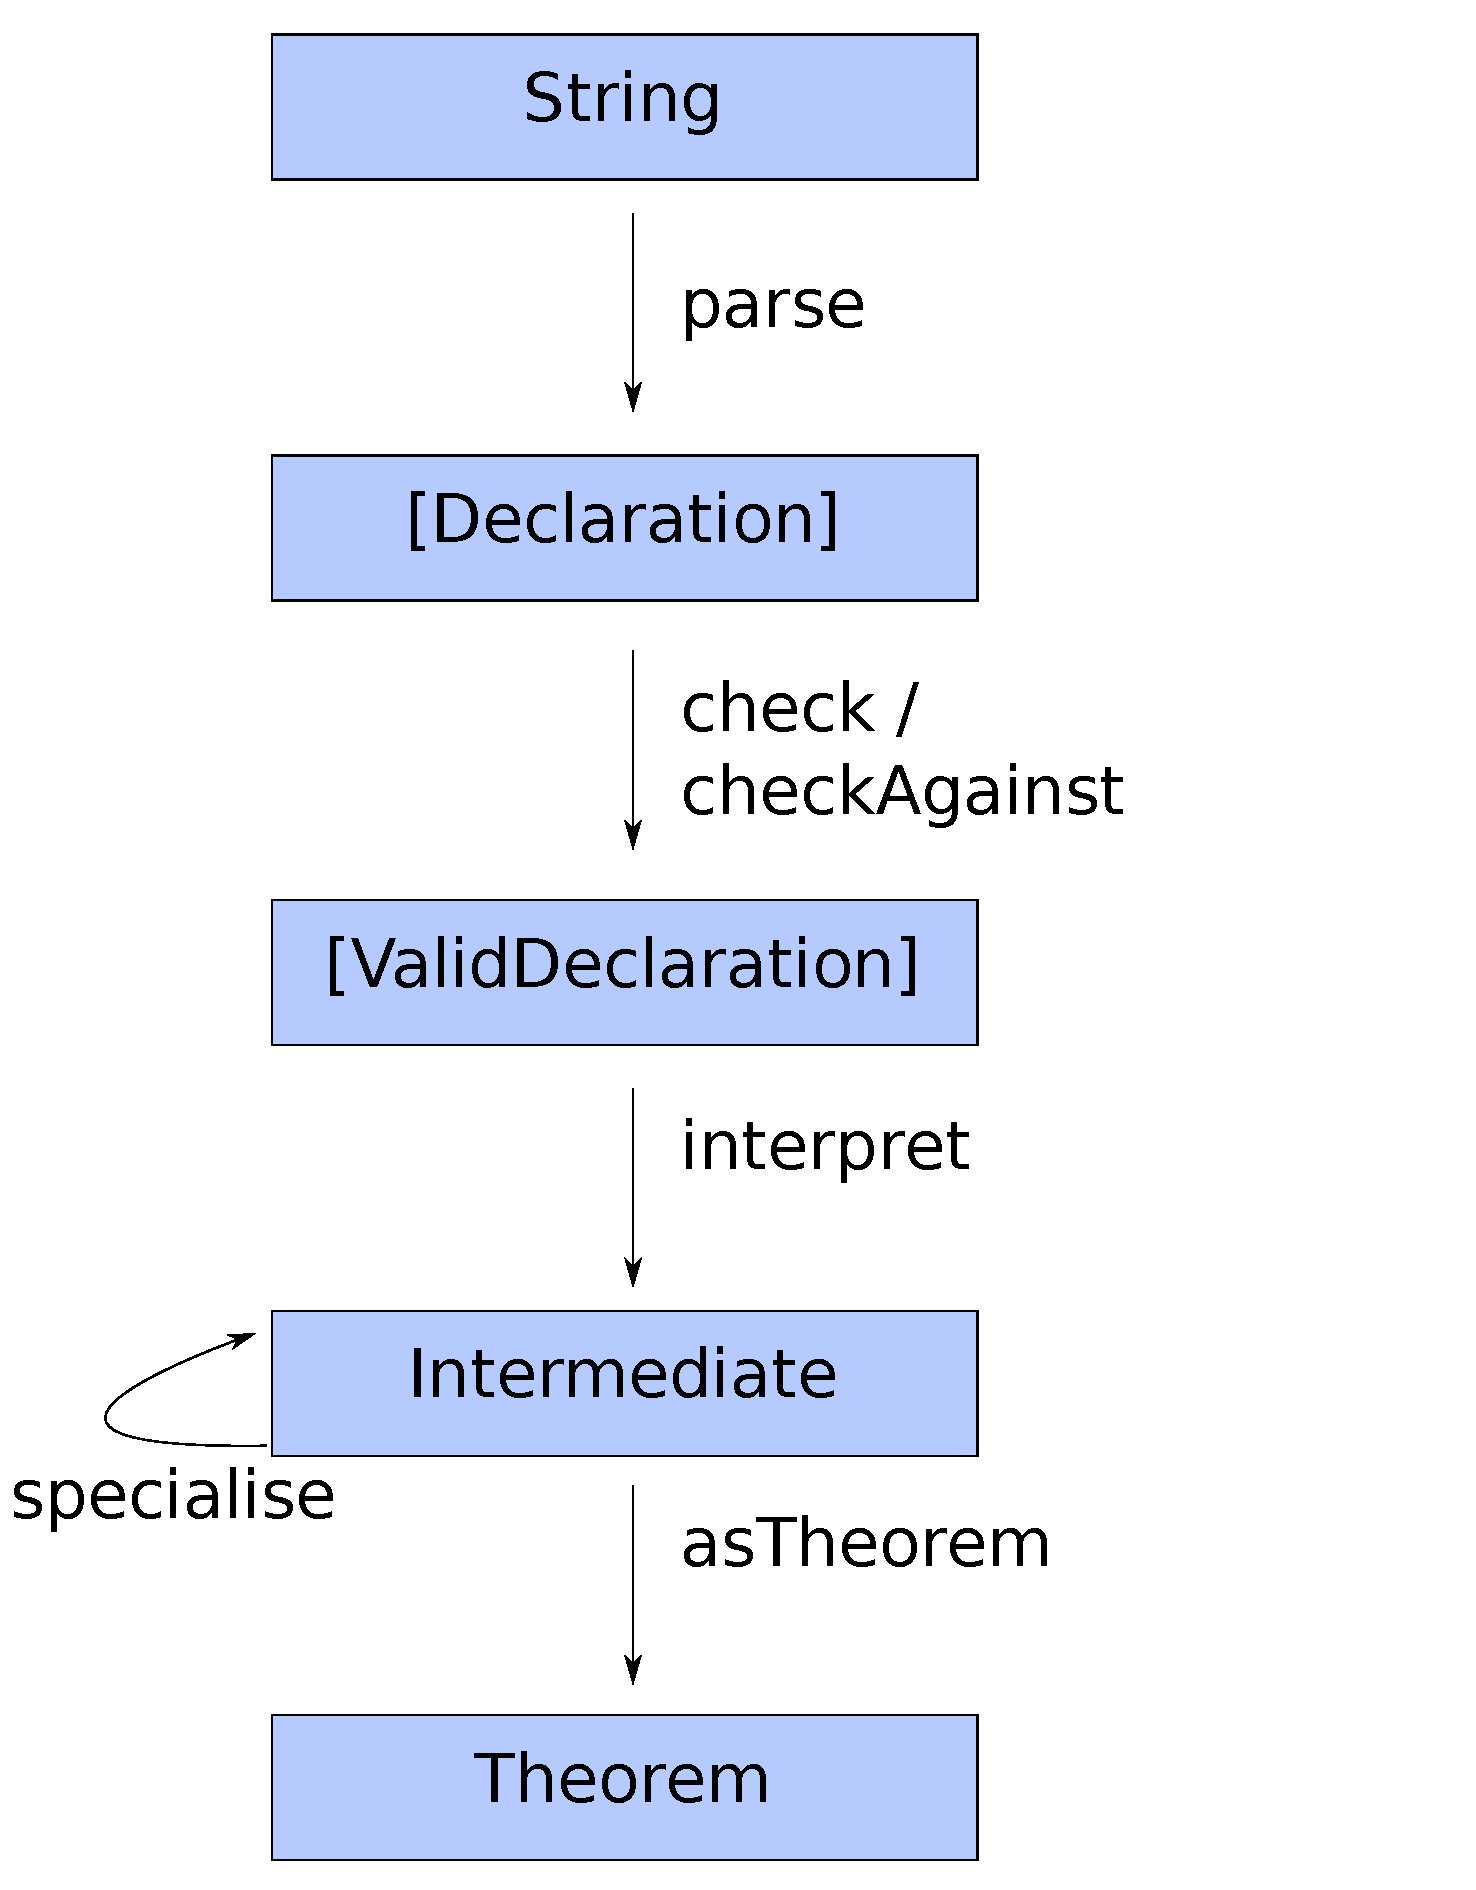
\includegraphics[height=200px]{overview-free-theorems}
     \end{center}
\end{column}
\begin{column}{0.6\textwidth}
  \begin{itemize}[<+->]
    \item parse: Erlaube Applikation von Typ(konstruktor)variablen
    \item check: Zusätzliche Checks benötigt
    \item interpret: Überführe Typvariablen-Applikation in entsprechende Relation
    \item asTheorem: Zusätzliche Abroll-Aktionen
    \item Erweiterung des Pretty Printers
  \end{itemize}
\end{column}
\end{columns}
\end{frame}

\begin{frame}
\frametitle{Die harte Realität}

\begin{itemize}
\item Nichtterminierung, Exceptions etc.
\item Striktheit
\item In free-theorem durch ``Language Subsets'' aufgeteilt
\end{itemize}

\end{frame}

\section{Zu tun}

\begin{frame}
\frametitle{Zu tun}

\begin{itemize}
\item Anpassen der Bibliothek an aktuelle GHC Versionen
\item Erweiterung der Datenstrukturen
\item Erweiterung der Bibliotheksfunktionen
\item Zusätzliche Local- und Global-Checks
\item Zusätzliche Aussagen zu speziellen Typklassen?
\item Zusätzliche Vereinfachungen?
\item Language Subsets beachten
\item Fehlerprüfung (Quickchecks erweitern)
\end{itemize}

\end{frame}

  \begin{frame}
  \vfill
  \centering
  \begin{beamercolorbox}[sep=8pt,center,shadow=true,rounded=true]{title}
    \usebeamerfont{title}Vielen Dank für die Aufmerksamkeit\par%
  \end{beamercolorbox}
  \vfill
  \end{frame}

\end{document}